\documentclass[a4paper]{article}

%·······························································································
%                                _    _                _           
%                               | |  | |              | |          
%                               | |__| | ___  __ _  __| | ___ _ __ 
%                               |  __  |/ _ \/ _` |/ _` |/ _ \ '__|
%                               | |  | |  __/ (_| | (_| |  __/ |   
%                               |_|  |_|\___|\__,_|\__,_|\___|_|   
%·······························································································

% Packages import
\usepackage[spanish]{babel}     % Spanish language support
\usepackage[utf8]{inputenc}     % UTF-8 encoding
\usepackage[T1]{fontenc}        % Proper font encoding
\usepackage{geometry}           % Page layout
\usepackage{titlesec}           % Custom section titles
\usepackage{lmodern}            % Modern font
\usepackage{fancyhdr}           % Header and footer
\usepackage{graphicx}           % Inserting images
\usepackage{anyfontsize}        % Arbitrary font size
\usepackage{listings}           % Code formatting
\usepackage{caption}            % Caption customizing
\usepackage{float}              % Image placing
\usepackage[colorlinks=true, linkcolor=black, urlcolor=Emerald]{hyperref}
\usepackage[dvipsnames]{xcolor}

% Packages configurations {{{

    % Adjust margins
    \geometry{a4paper, margin=2.5cm}
    
    % Change default command to resize all text
    \renewcommand{\normalsize}{\fontsize{13}{16}\selectfont}
    
    % Header/Footer settings
    \fancyfoot[C]{\thepage}

    % Shell prompt code
    \lstdefinestyle{shellprompt}{
        backgroundcolor=\color{black},
        basicstyle=\fontsize{11}{20}\ttfamily\color{white},
        keywordstyle=\color{NavyBlue},
        commentstyle=\color{white},
        stringstyle=\color{green},
        breaklines=true,
    }

    % Define the style for code with line numbers
    \lstdefinestyle{normalcode}{
        numbers=left,         % Display line numbers on the left
        numberstyle=\tiny,    % Small size for the line numbers
        stepnumber=1,         % Number every line
        numbersep=5pt,        % Space between line numbers and code
        backgroundcolor=\color{lightgray}, % Background color of code block
        basicstyle=\ttfamily\footnotesize, % Set font to typewriter and small size
    }

    % Set default listings style to shellprompt
    \lstset{style=shellprompt}

% }}}

\hyphenpenalty=10000  % Avoid hyphenation
\exhyphenpenalty=10000
\sloppy  % Loosens the strictness of the justification algorithm

% Metadata {{{

    % Title
    \title{Sistemas Cooperativos y Gestión de Contenidos}
    
    % Author
    \author{Juan Manuel Segura Duarte}

% }}}



%·······························································································
%                     _____                                        _   
%                    |  __ \                                      | |  
%                    | |  | | ___   ___ _   _ _ __ ___   ___ _ __ | |_ 
%                    | |  | |/ _ \ / __| | | | '_ ` _ \ / _ \ '_ \| __|
%                    | |__| | (_) | (__| |_| | | | | | |  __/ | | | |_ 
%                    |_____/ \___/ \___|\__,_|_| |_| |_|\___|_| |_|\__|
%·······························································································
\begin{document}

% Cover Page
\begin{titlepage}
    \centering
    \vspace*{3cm}  % Space at the top
    {\Huge \textbf{SCGC Práctica 1}} % Custom title
    \vspace{1cm}
    
    {\Large Sistemas Cooperativos y Gestión de Contenidos: Desarrollo de la 1ª práctica} % Subtitle
    
    
\includegraphics[width=0.5\textwidth]{images/ugr_logo.png}
    \vspace{1cm}
    
    \textbf{\Large Juan Manuel Segura Duarte} % Author name
\end{titlepage}
\newpage

% Table of Contents page
\thispagestyle{empty}
\tableofcontents

%%%%%%%%%%%%%%%%%%%%%%%%%%%%%%%%%%%%%%%%%%%%%%%%%%%%%%%%%%%%%%%%%%%%%%%%%%%%%%%%%%%%%%%%%%%%%%%%%%
%%%%%%%%%%%%%%%%%%%%%%%%%%%%%%%%%%%%%%%%%%%%%%%%%%%%%%%%%%%%%%%%%%%%%%%%%%%%%%%%%%%%%%%%%%%%%%%%%%
%%%%%%%%%%%%%%%%%%%%%%%%%%%%%%%%%%%%%%%%%%%%%%%%%%%%%%%%%%%%%%%%%%%%%%%%%%%%%%%%%%%%%%%%%%%%%%%%%%

% Start numbering in this page (after the title page and index)
\newpage
\pagenumbering{arabic}
\setcounter{page}{1}

\section{Propuesta de trabajo}

En este trabajo se llevará a cabo la configuración de un entorno de desarrollo local para el stack LAMP (Linux, Apache, MySQL, PHP) utilizando Docker Compose. Se utilizará un enfoque manual para la configuración del archivo \texttt{docker-compose.yaml} para tener mayor flexibilidad y control sobre cada componente del sistema.

\vspace{1em}

El enfoque propuesto implica el uso de contenedores individuales para la aplicación WordPress (que incorpora Apache y PHP) y para MySQL, permitiendo una administración más granular y la capacidad de actualizar componentes específicos sin afectar al entorno completo. Esto también facilita la persistencia de datos a través de volúmenes Docker, garantizando que los datos se mantengan a salvo incluso al reconstruir los contenedores.

\vspace{1em}

Se proporcionará una guía detallada sobre la configuración del archivo \texttt{docker-compose.yaml}, la creación de volúmenes persistentes y la instalación de WordPress como CMS, destacando la importancia de mantener un entorno de desarrollo reproducible y escalable.

\vspace{2em}

\begin{figure}[!h]
    \centering
    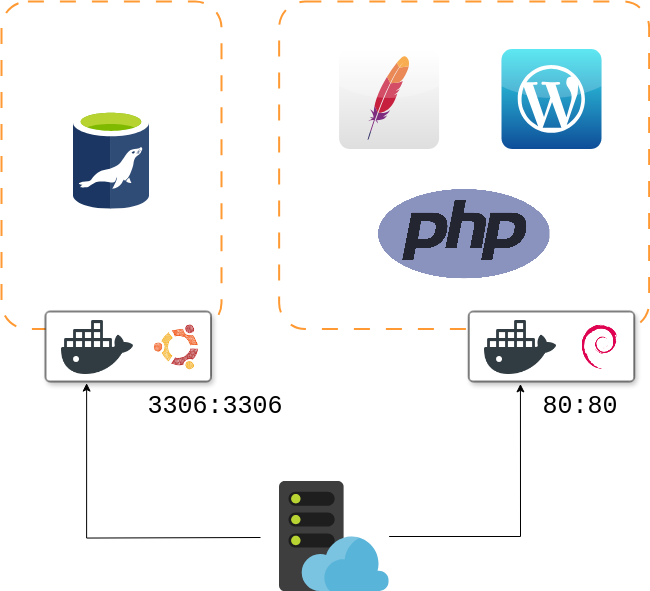
\includegraphics[width=0.75\textwidth]{images/lamp_docker_diagram.png}
    \captionsetup{width=0.7\textwidth}
    \caption{Esquema de la arquitectura empleada para el servidor.}
    \label{fig:lamp_stack}
\end{figure}

\newpage

%%%%%%%%%%%%%%%%%%%%%%%%%%%%%%%%%%%%%%%%%%%%%%%%%%%%%%%%%%%%%%%%%%%%%%%%%%%%%%%%%%%%%%%%%%%%%%%%%%
%%%%%%%%%%%%%%%%%%%%%%%%%%%%%%%%%%%%%%%%%%%%%%%%%%%%%%%%%%%%%%%%%%%%%%%%%%%%%%%%%%%%%%%%%%%%%%%%%%
%%%%%%%%%%%%%%%%%%%%%%%%%%%%%%%%%%%%%%%%%%%%%%%%%%%%%%%%%%%%%%%%%%%%%%%%%%%%%%%%%%%%%%%%%%%%%%%%%%

\section{Configuración del sistema}

Debido al extendido uso de Docker hoy en día, no es dificil encontrar imágenes o archivos \texttt{docker-compose.yaml} que se ajusten a nuestras necesidades. Si buscamos en internet imágenes que tengan Wordpress encontraremos que hay imagenes oficiales con gran parte de lo que necesitamos, \texttt{php} y \texttt{apache}.

\begin{figure}[!h]
    \centering
    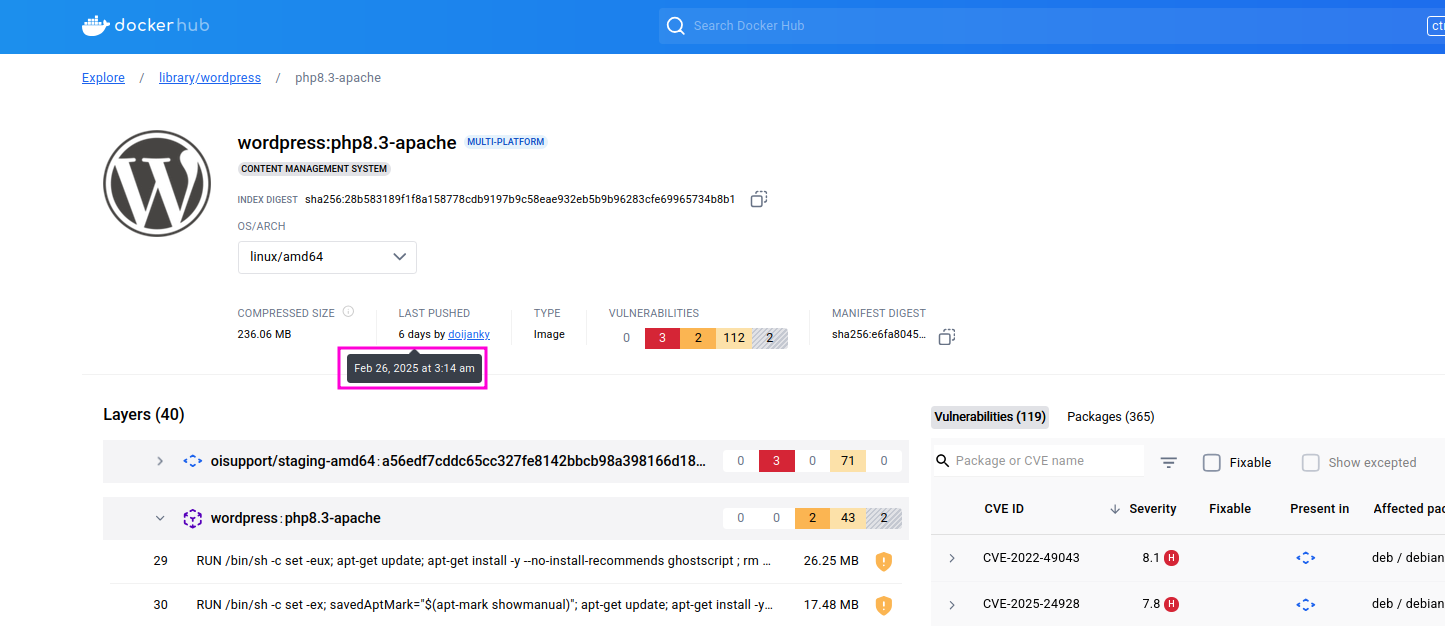
\includegraphics[width=0.9\textwidth]{images/docker_hub_wordpress.png}
    \caption{Imagen oficial de WordPress en Docker Hub. \href{https://hub.docker.com/layers/library/wordpress/php8.3-fpm/images/sha256-1841db5f891825b1c279bf170338cb17f868f1ef257fa2cd73ad2c2ed2cb9b0e}{Enlace}}
    \label{fig:docker_wordpress}
\end{figure}

\vspace{1em}

Además, debido a la popularidad de ambos el stack LAMP y el CMS Wordpress, existen ejemplos oficiales de Docker en el que se realiza justo esto (si se utiliza la imagen de Wordpress con php y apache). En este caso se ha utilizado \texttt{docker-compose.yaml} se ha utilizado \href{https://github.com/docker/awesome-compose/blob/master/official-documentation-samples/wordpress/README.md}{este ejemplo oficial} como base para nuestro docker-compose.yaml. Para tener un cliente gráfico SQL desde el que poder hacer queries al servidor solo es necesario añadir otro servicio al archivo compose \href{https://hub.docker.com/_/phpmyadmin}{utilizando una imagen como esta}. Este servicio (contenedor) no se encuentra representado en el diagrama ya que no forma parte de la arquitectura en sí, habiendo expuesto el puerto 3306 del contenedor de la BD (Base de Datos) se puede utilizar cualquier SGBD (Sistema Gestor de Bases de Datos), como podría ser una instalación local de phpMyAdmin, o la propia CLI (Command Line Interface) que proporciona MariaDB en el host (se podría conectar usando el comando \\ \texttt{mariadb -h 127.0.0.1 -P \$EXPOSED\_PORT -u \$DB\_USER -p}).

\vspace{1em}

Los pasos a seguir para la creación del entorno son los siguientes:

\begin{enumerate}
    \item Crear un nuevo directorio para el proyecto:
    \begin{lstlisting}
touch docker-compose.yaml
    \end{lstlisting}

    \newpage

    \item Crear el archivo \texttt{docker-compose.yaml} con el siguiente contenido:
    \begin{lstlisting}
version: '3.1'

services:
  db:
    image: mariadb:11.7.2-noble
    restart: always
    volumes:
      - db_data:/var/lib/mysql
    environment:
      - MARIADB_ROOT_PASSWORD=<MARIADB_ROOT_PASSWORD>
      - MARIADB_DATABASE=wordpress_db
      - MARIADB_USER=wordpressAdmin
      - MARIADB_PASSWORD=<MARIADB_USER_PASSWORD>
    ports:
      - 3306:3306

  wordpress:
    image: wordpress:6.7.2-php8.1-apache
    restart: always
    volumes:
      - wp_data:/var/www/html
    ports:
      - 80:80
    environment:
      - WORDPRESS_DB_HOST=db:3306
      - WORDPRESS_DB_USER=wordpressAdmin
      - WORDPRESS_DB_PASSWORD=<MARIADB_USER_PASSWORD (same as MARIADB_PASSWORD)>
      - WORDPRESS_DB_NAME=wordpress_db
    depends_on:
      - db

  phpmyadmin:
    image: phpmyadmin:5.2.2-apache
    restart: always
    ports:
      - 8080:80
    environment:
      - PMA_HOST=db:3306
      - MYSQL_ROOT_PASSWORD=<MARIADB_ROOT_PASSWORD>
      - MYSQL_USER=wordpressAdmin
      - MYSQL_PASSWORD=<MARIADB_USER_PASSWORD (same as MARIADB_PASSWORD)>
    depends_on:
      - db

volumes:
  db_data:
  wp_data:
    \end{lstlisting}
    Véase \href{https://hub.docker.com/_/mariadb}{la sección de variables de entorno en la página de la imagen de Docker de MariaDB}, la cual contiene las variables más usadas comentadas brevemente y, más completamente, \href{https://mariadb.com/kb/en/mariadb-server-docker-official-image-environment-variables/}{la referencia de variables de MariaDB}. Cabe destacar también \href{https://hub.docker.com/_/wordpress}{la documentación sobre Wordpress que viene en su página oficial de Docker}.

    \item Crear la estructura de directorios necesaria:
    \begin{lstlisting}
mkdir wp_data db_data
    \end{lstlisting}

    \item Iniciar los contenedores:
    \begin{lstlisting}
docker compose up
    \end{lstlisting}

    \item Acceder a la aplicación en el navegador \texttt{localhost} lo que nos lleva a la instalación de Wordpress

    \begin{figure}[!h]
        \centering
        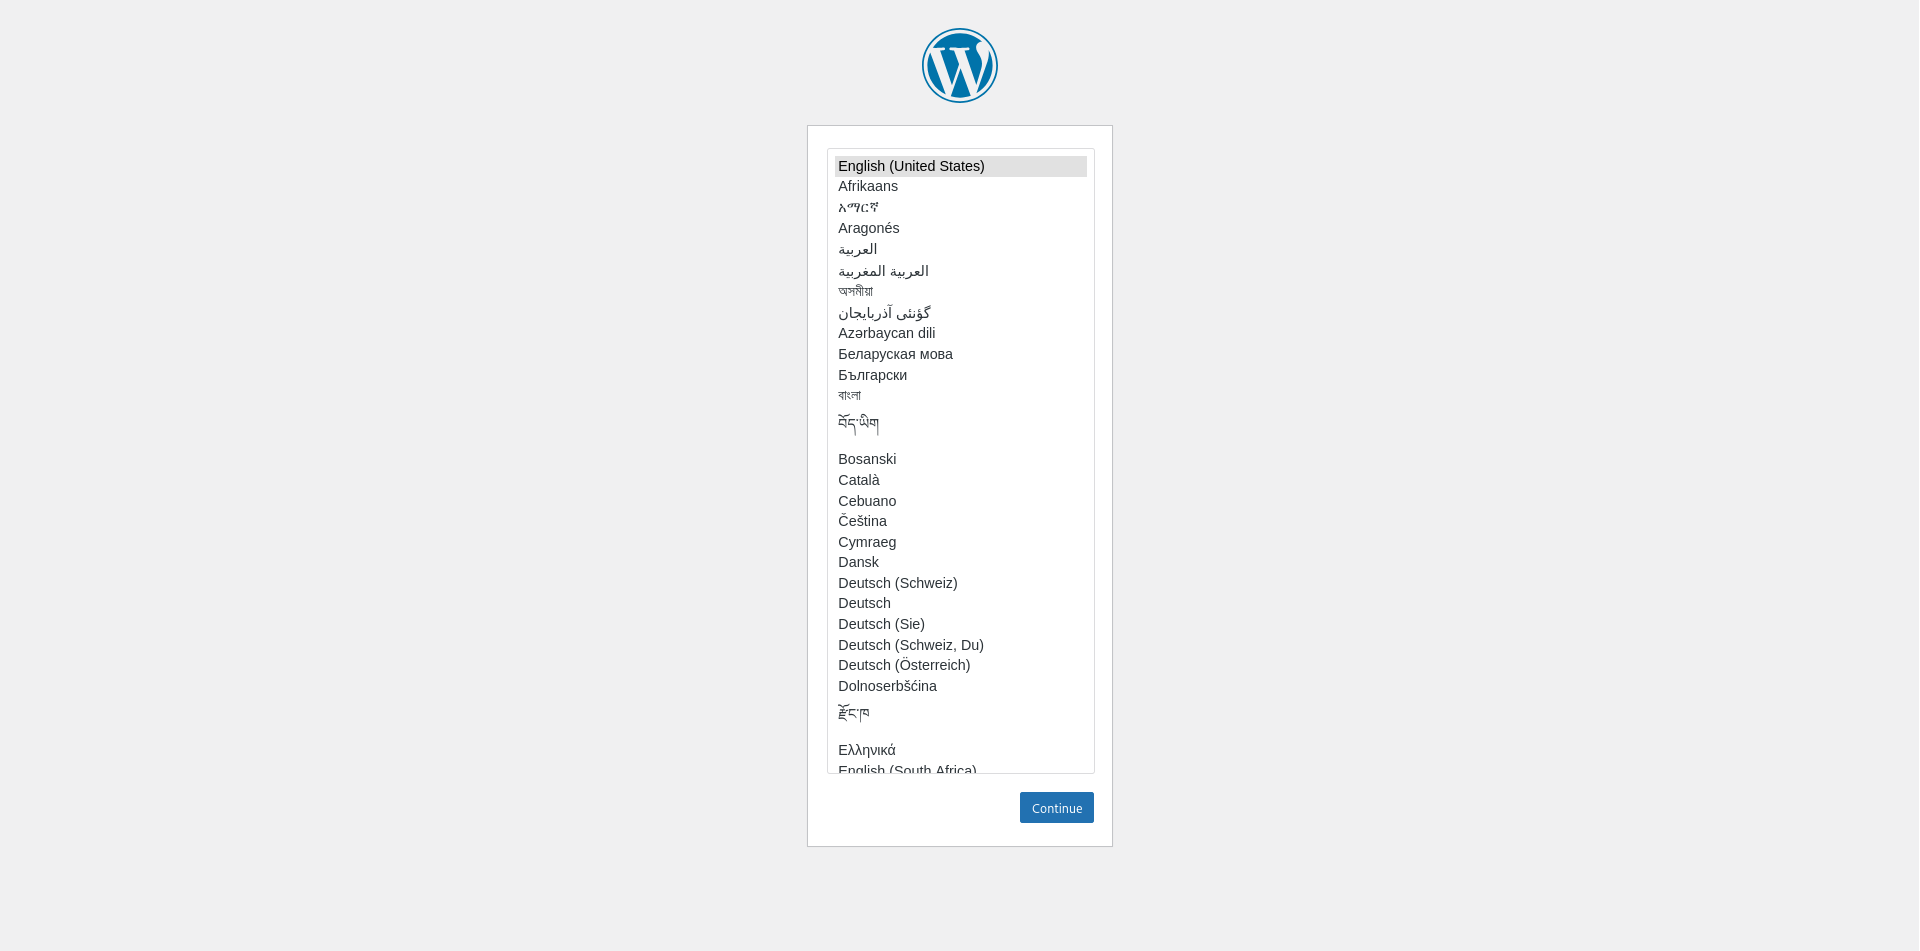
\includegraphics[width=0.8\linewidth]{images/wp_install1.png}
    \end{figure}
    
\end{enumerate}

%%%%%%%%%%%%%%%%%%%%%%%%%%%%%%%%%%%%%%%%%%%%%%%%%%%%%%%%%%%%%%%%%%%%%%%%%%%%%%%%%%%%%%%%%%%%%%%%%%
%%%%%%%%%%%%%%%%%%%%%%%%%%%%%%%%%%%%%%%%%%%%%%%%%%%%%%%%%%%%%%%%%%%%%%%%%%%%%%%%%%%%%%%%%%%%%%%%%%
%%%%%%%%%%%%%%%%%%%%%%%%%%%%%%%%%%%%%%%%%%%%%%%%%%%%%%%%%%%%%%%%%%%%%%%%%%%%%%%%%%%%%%%%%%%%%%%%%%

\newpage

\section{Instalación de Wordpress}

\begin{enumerate}

    \item Lo retomamos donde lo dejamos en el paso anterior, con la pantalla para seleccionar el idioma, aquí vamos a seleccionar inglés debido a su relevancia en el mundo de la informática y las ingenierías en general.
    \begin{figure}[!h]
        \centering
        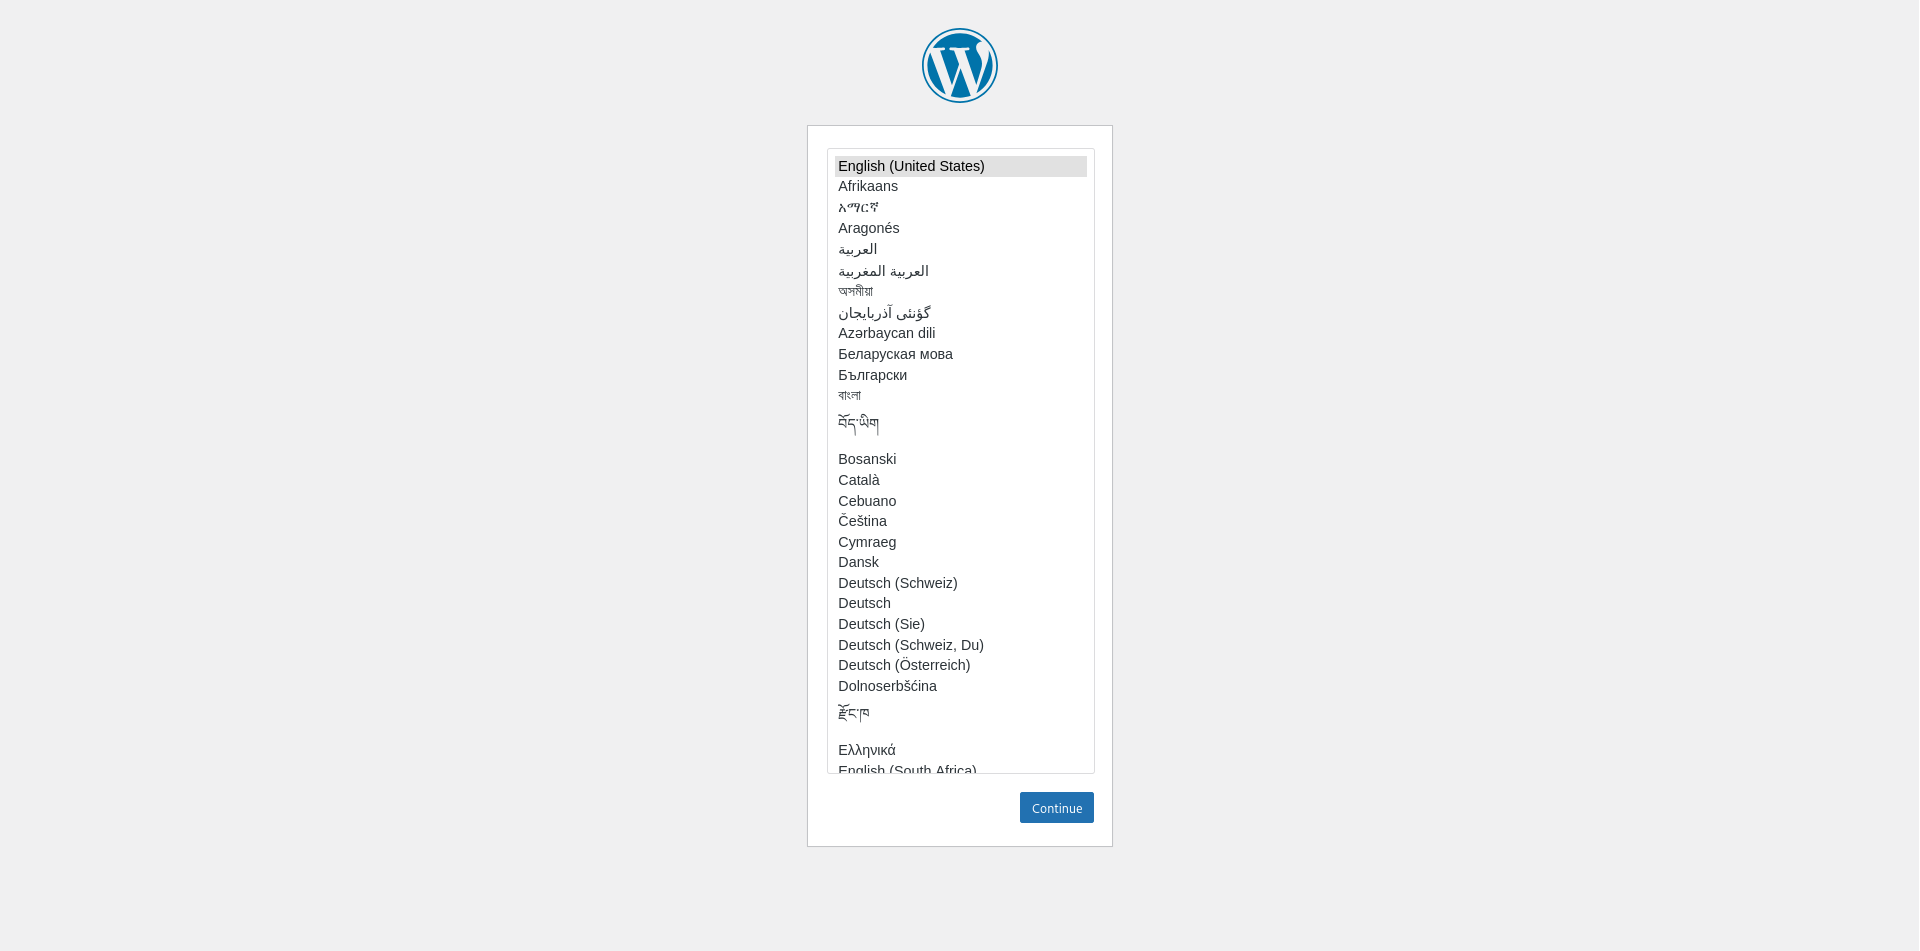
\includegraphics[width=0.8\linewidth]{images/wp_install1.png}
    \end{figure}

    \item Rellenamos los datos solicitados.
    \begin{figure}[!h]
        \centering
        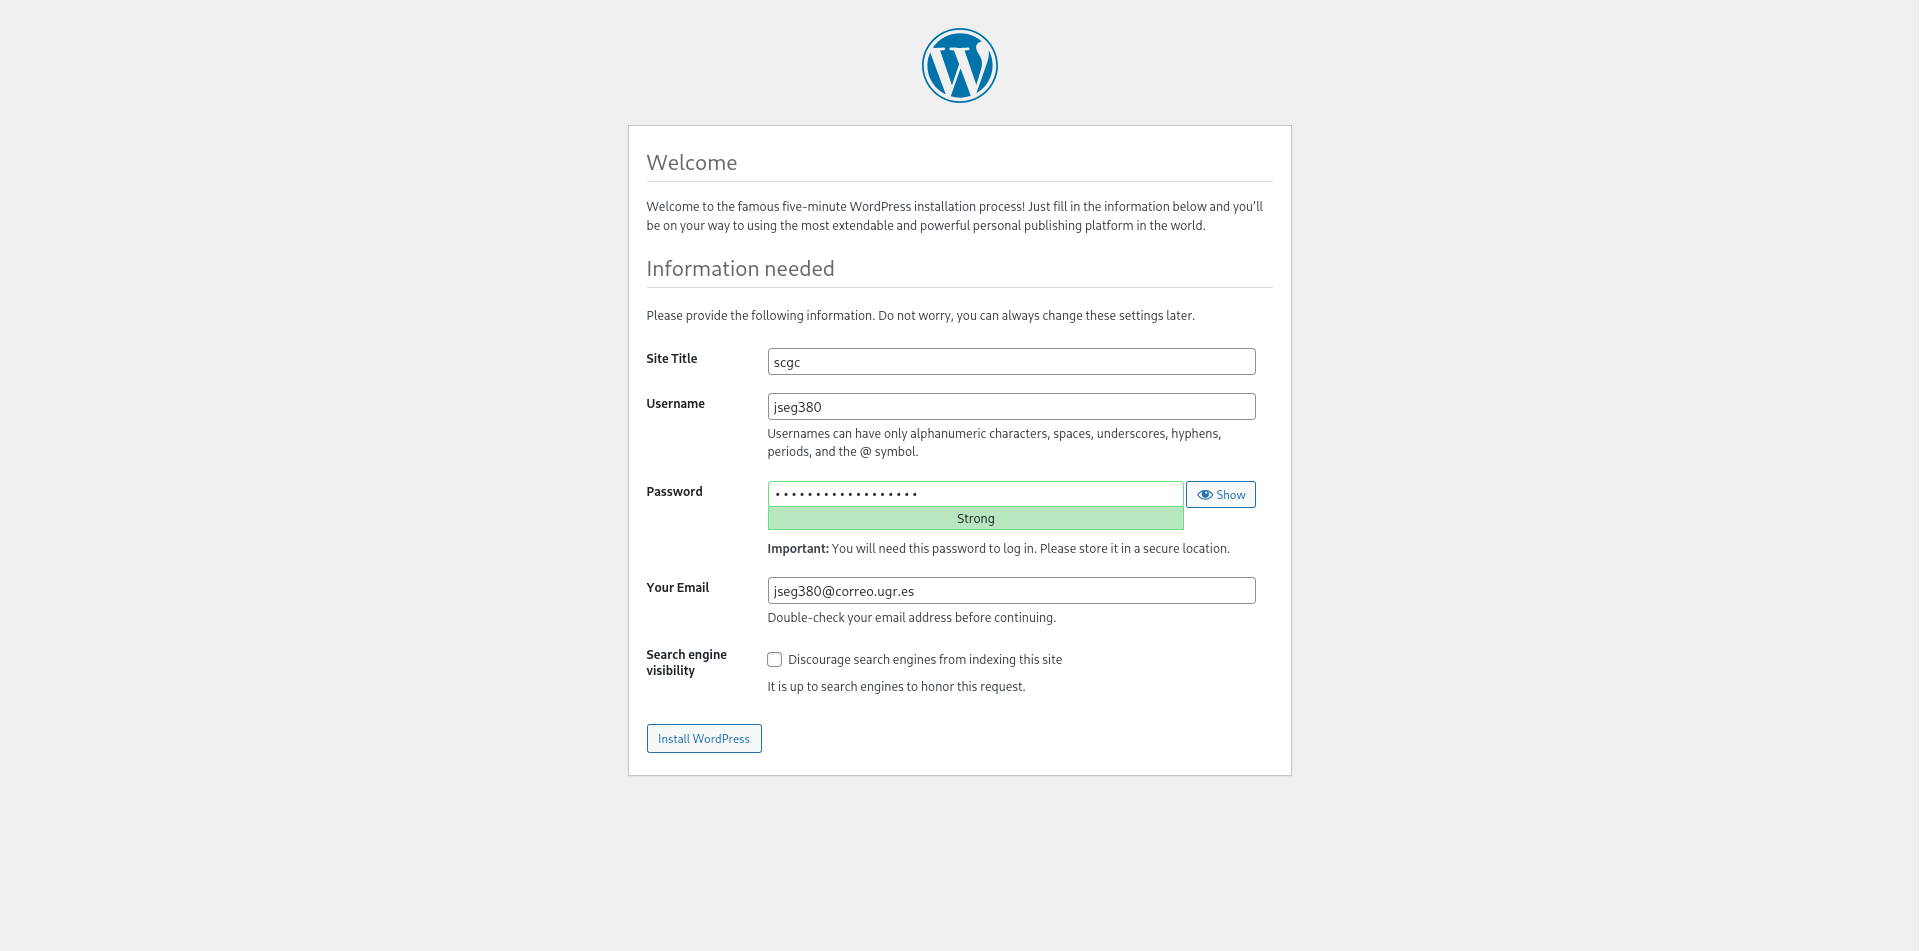
\includegraphics[width=0.8\linewidth]{images/wp_install2.png}
    \end{figure}
    \begin{figure}[!h]
        \centering
        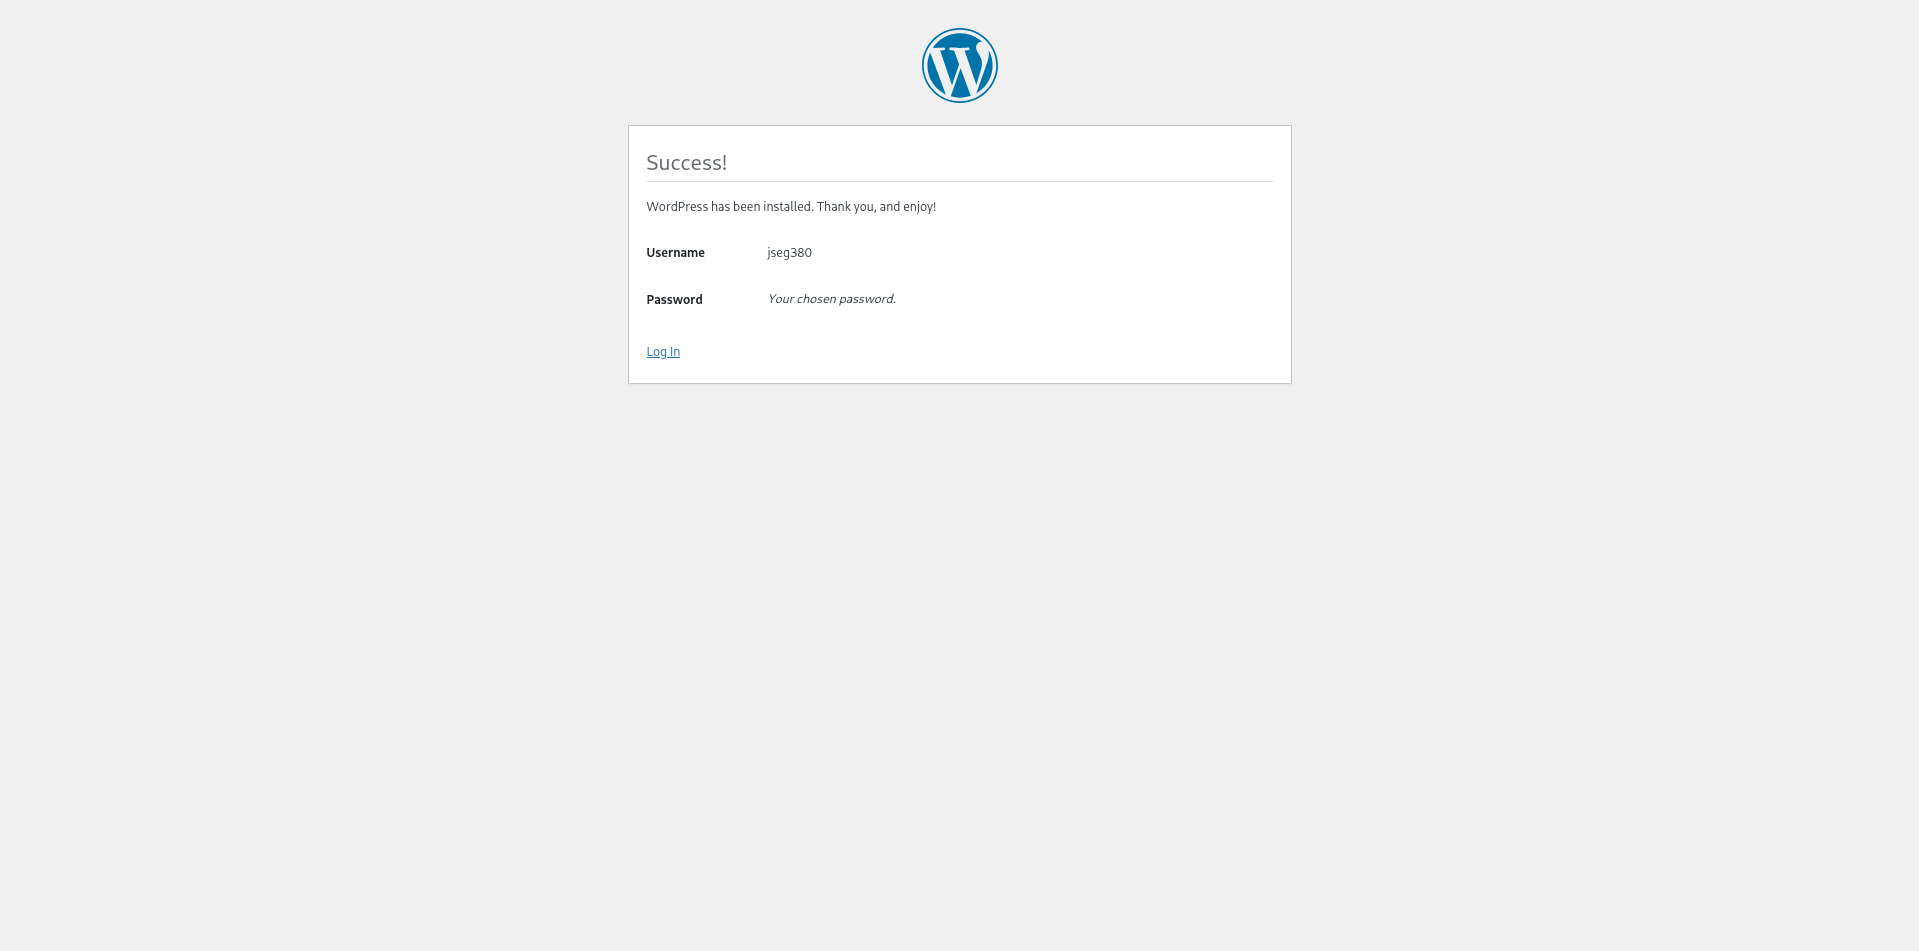
\includegraphics[width=0.8\linewidth]{images/wp_install3.png}
    \end{figure}

    \item Después nos llevará al login, en el que introducimos los datos seleccionados anteriormente.
    \begin{figure}[!h]
        \centering
        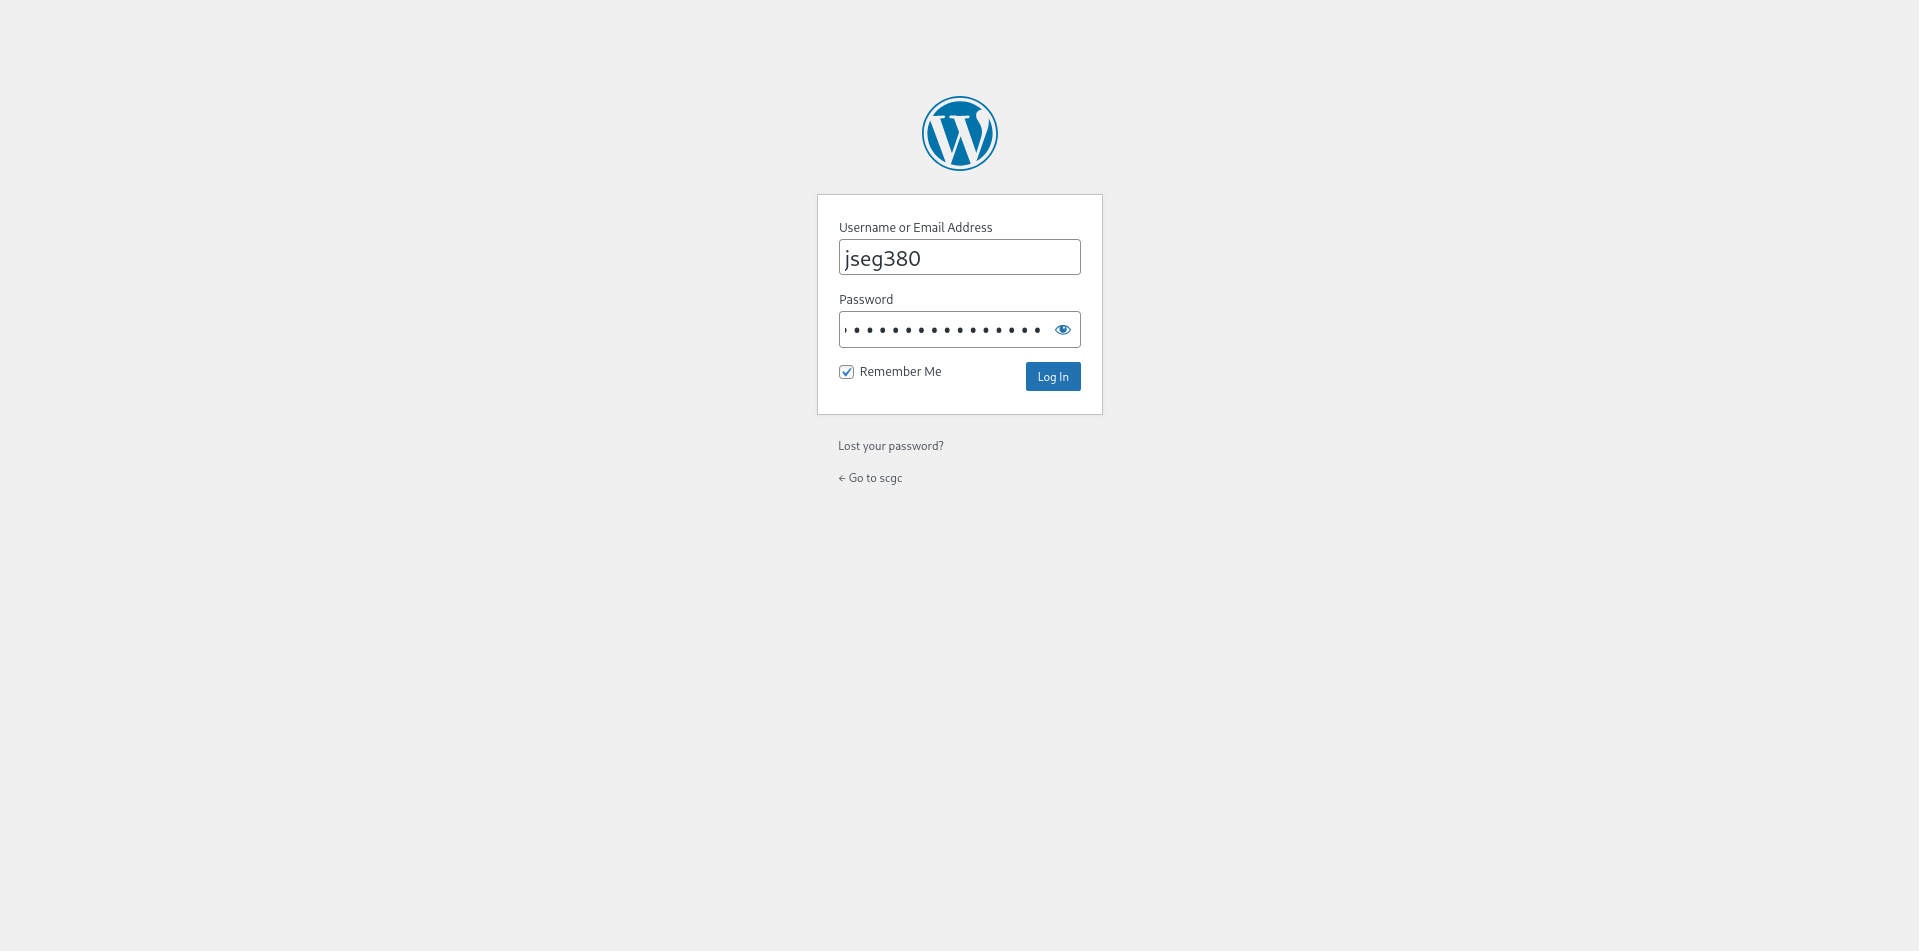
\includegraphics[width=0.8\linewidth]{images/wp_install4.png}
    \end{figure}
    \begin{figure}[!h]
        \centering
        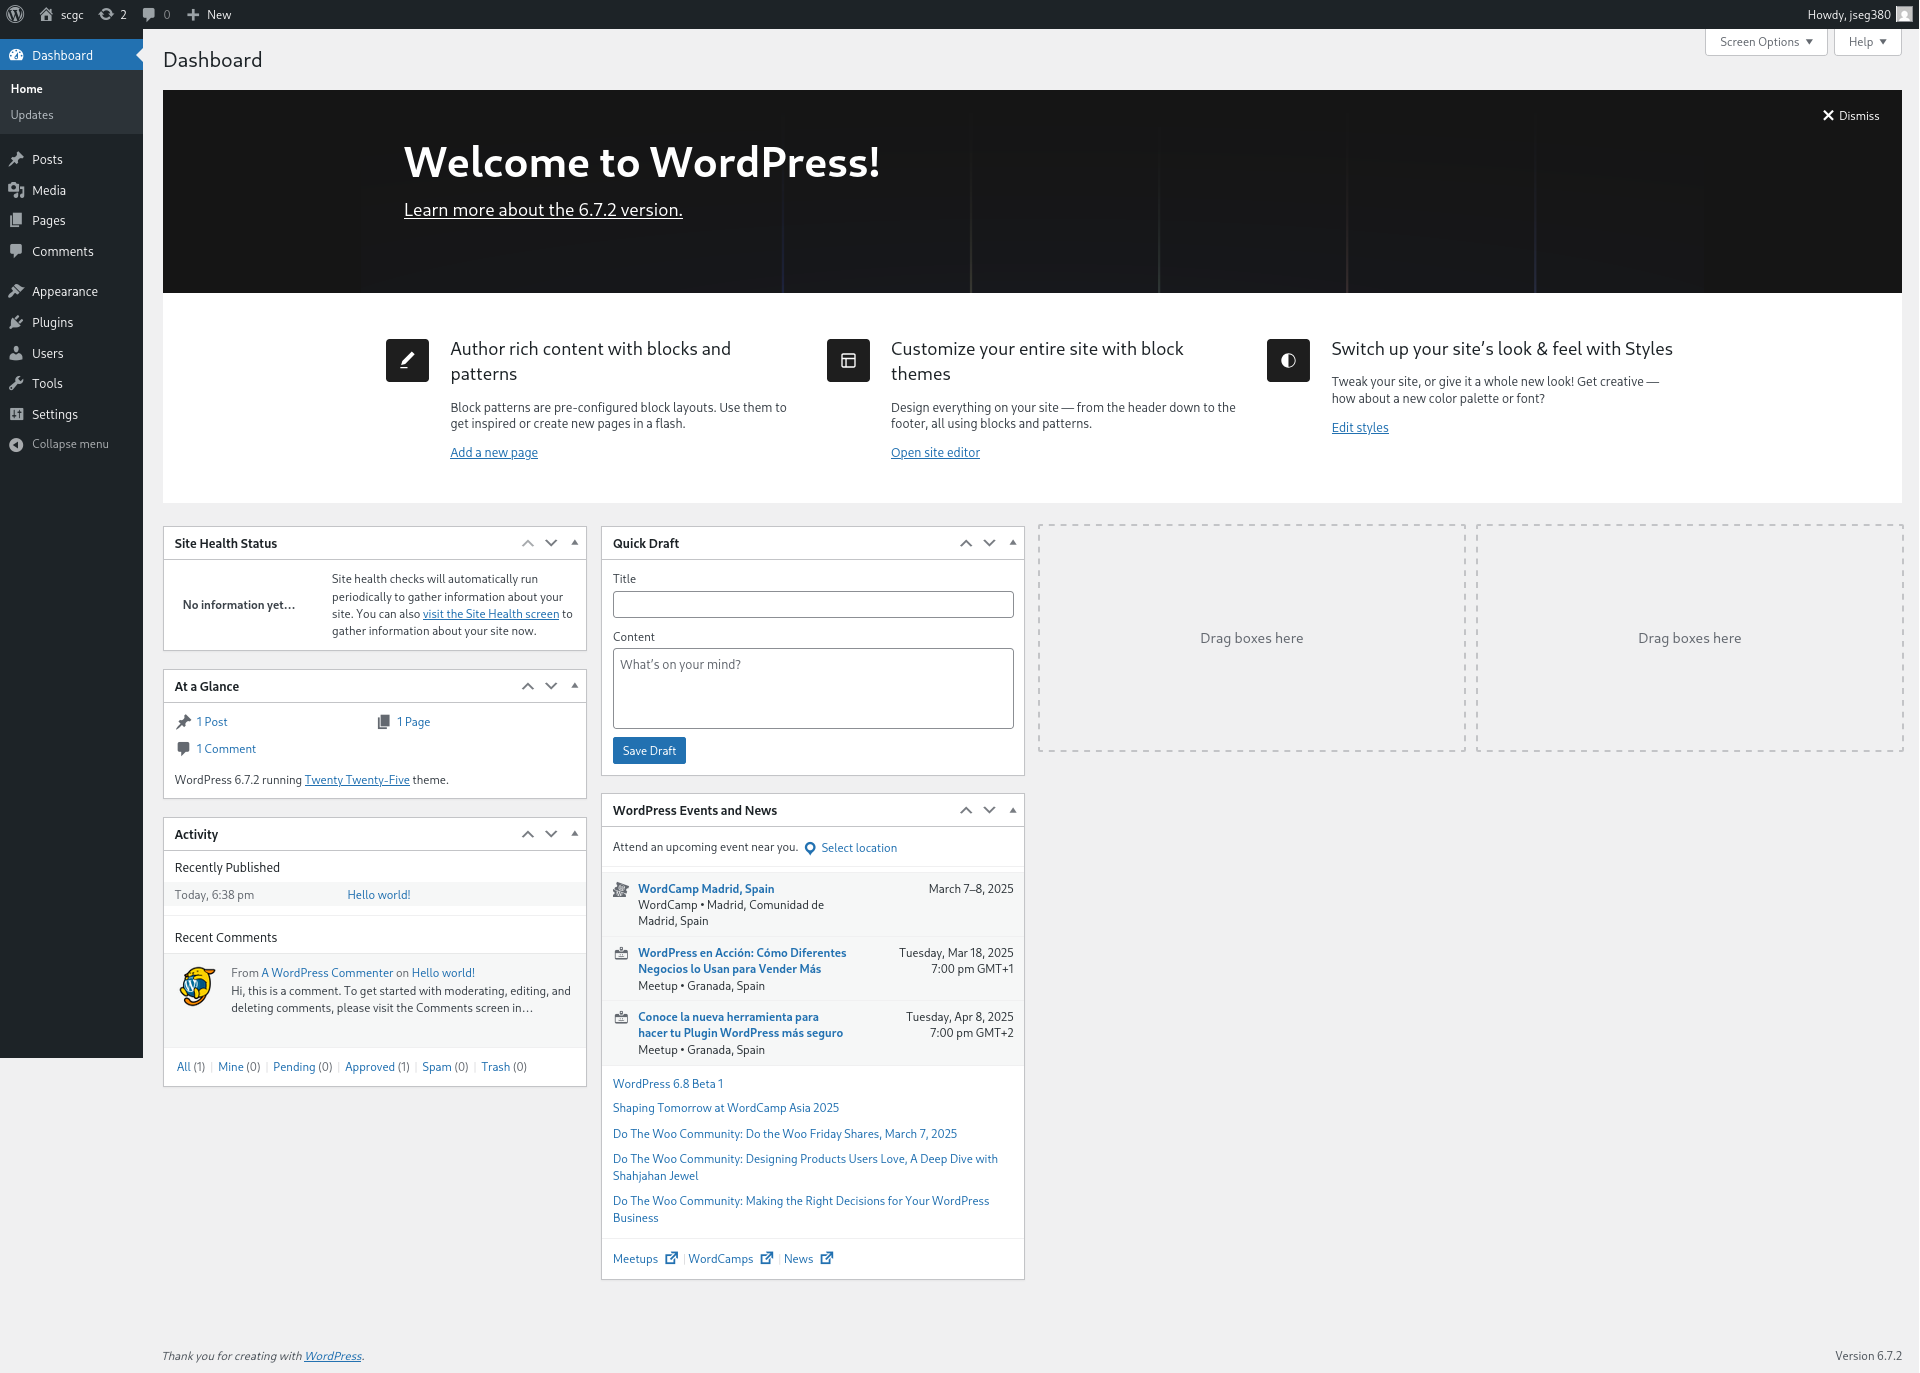
\includegraphics[width=0.8\linewidth]{images/wp_install5.png}
    \end{figure}
        
\end{enumerate}

%%%%%%%%%%%%%%%%%%%%%%%%%%%%%%%%%%%%%%%%%%%%%%%%%%%%%%%%%%%%%%%%%%%%%%%%%%%%%%%%%%%%%%%%%%%%%%%%%%
%%%%%%%%%%%%%%%%%%%%%%%%%%%%%%%%%%%%%%%%%%%%%%%%%%%%%%%%%%%%%%%%%%%%%%%%%%%%%%%%%%%%%%%%%%%%%%%%%%
%%%%%%%%%%%%%%%%%%%%%%%%%%%%%%%%%%%%%%%%%%%%%%%%%%%%%%%%%%%%%%%%%%%%%%%%%%%%%%%%%%%%%%%%%%%%%%%%%%

\section{Conclusión}

La configuración manual del stack utilizando Docker Compose permite un control total sobre el entorno de desarrollo. Al emplear un contenedor para la aplicación WordPress (que integra Apache y PHP) y otro para MySQL, se facilita la administración, la seguridad y la escalabilidad del sistema. Además, la persistencia de datos mediante volúmenes asegura que el progreso del proyecto no se vea afectado por posibles reconstrucciones de los contenedores. El enfoque propuesto proporciona una solución flexible y eficiente para el desarrollo de aplicaciones web basadas en WordPress.

\end{document}
